\documentclass[a4paper,10pt]{article}
\usepackage{parskip}
\usepackage[utf8]{inputenc}
\usepackage[english]{babel}
\usepackage[T1]{fontenc}
%\usepackage[top=2cm,bottom=2cm,left=2cm,right=2cm]{geometry}
\usepackage{enumerate}
\usepackage{graphicx}
%\usepackage[table,xcdraw]{xcolor}
\usepackage[usenames,dvipsnames]{xcolor}
%\usepackage{color}
\usepackage{caption}
\usepackage{listings}
\usepackage[pdftex]{hyperref}
\usepackage{fancyhdr} % Required for custom headers
\usepackage{lastpage} % Required to determine the last page for the footer
\usepackage{extramarks} % Required for headers and footers
\usepackage{mathtools}
\usepackage{color}
\usepackage{todonotes}

\definecolor{mygreen}{rgb}{0,0.6,0}
\definecolor{mygray}{rgb}{0.5,0.5,0.5}
\definecolor{mymauve}{rgb}{0.58,0,0.82}

\usepackage{array}
\usepackage{float}
\author{Groupe 30}
\title{Machine Learning - Assignment 4}
\date{\today}

% Margins
%\topmargin=-0.45in
%\textwidth=6.5in
%\textheight=9.8in
\headsep=0.25in
\headheight=13pt
% Set up the header and footer
%\pagestyle{empty}
\rhead{\firstxmark}
 % Top right header
\lfoot{\lastxmark} % Bottom left footer
\cfoot{} % Bottom center footer
\rfoot{Page\ \thepage\ /\ \protect\pageref{LastPage}} % Bottom right footer
\renewcommand\headrulewidth{0.3pt} % Size of the header rule
\renewcommand\footrulewidth{0.3pt} % Size of the footer rule

%\setlength\parindent{0pt} % Removes all indentation from paragraphs


\begin{document}

%\hypersetup{pageanchor=false}
\definecolor{lightyellow}{HTML}{FFFBEF}

\begin{titlepage}
\newcommand{\HRule}{\rule{\linewidth}{0.5mm}}

\includegraphics[width=6cm,height=1.9cm]{images/Logo_EPL.jpg}
\hfill

\includegraphics[width=3.3 cm,height=2.2 cm]{images/ucl.jpg}
%Defines a new command for the horizontal lines, change thickness here

\centering % Center everything on the page

%	HEADING SECTIONS
\null
\vspace{4 cm}

%	TITLE SECTION

\HRule \\[0.9cm]

{ {\LARGE LSINF2335 - Programming paradigms}\\[0.4cm]

\huge \textbf{Report} \\[0.6 cm]
% Title of your document
{\LARGE \textsc{A Comparison of \\ Reflection \& Meta-programming \\
in \\
Python and JavaScript} }}
\\[0.9cm]
\HRule \\[2cm]

\Large {

\begin{tabular}{rl}
\multicolumn{2}{c}{\textbf{Group 1}}  \\[0.3 cm]
\textsc{Gerondal} & Thibault  \\
\textsc{Heraly } & Michaël \\



\end{tabular}}
\\[1.8cm]


%	DATE SECTION

\large{Academic year 2014 -- 2015} % Date, change the \today to a set date if you want to be precise

\end{titlepage}

%----------------------------------------------------------------------------------------
%	TABLE OF CONTENTS
%----------------------------------------------------------------------------------------

\pagenumbering{gobble}
\clearpage
\thispagestyle{empty}
\tableofcontents
\clearpage
\pagenumbering{arabic}
\newpage

%----------------------------------------------------------------------------------------
%	TEXT
%----------------------------------------------------------------------------------------

\newcommand{\setjs}{
    \lstdefinelanguage{JavaScript}{
      keywords={typeof, new, for, true, false, catch, function, return, null, Array, Regexp, catch, switch, var, if, in, while, do, else, case, break, this},
      keywordstyle=\color{blue}\bfseries,
      ndkeywords={class, export, throw, implements, import, this},
      ndkeywordstyle=\color{darkgray}\bfseries,
      identifierstyle=\color{black},
      %sensitive=false,
      comment=[l]{//},
      morecomment=[s]{/*}{*/},
      commentstyle=\color{mygreen}\ttfamily,
      stringstyle=\color{red}\ttfamily,
      morestring=[b]',
      morestring=[b]",
      tabsize=4,
    }
    \lstset{language=JavaScript}
}
\newcommand{\setpy}{\lstset{language=Python}
\lstset{ %
  backgroundcolor=\color{white},   % choose the background color; you must add \usepackage{color} or \usepackage{xcolor}
  basicstyle=\footnotesize\ttfamily,        % the size of the fonts that are used for the code
  breakatwhitespace=false,         % sets if automatic breaks should only happen at whitespace
  breaklines=true,                 % sets automatic line breaking
  captionpos=b,                    % sets the caption-position to bottom
  commentstyle=\color{mygreen},    % comment style
  deletekeywords={...},            % if you want to delete keywords from the given language
  escapeinside={\%*}{*)},          % if you want to add LaTeX within your code
  extendedchars=true,              % lets you use non-ASCII characters; for 8-bits encodings only, does not work with UTF-8
  frame=single,                    % adds a frame around the code
  keepspaces=true,                 % keeps spaces in text, useful for keeping indentation of code (possibly needs columns=flexible)
  keywordstyle=\color{blue},       % keyword style
  language=Octave,                 % the language of the code
  otherkeywords={*,\%,...},            % if you want to add more keywords to the set
  %numbers=left,                    % where to put the line-numbers; possible values are (none, left, right)
  numbersep=5pt,                   % how far the line-numbers are from the code
  numberstyle=\tiny\color{mygray}, % the style that is used for the line-numbers
  rulecolor=\color{black},         % if not set, the frame-color may be changed on line-breaks within not-black text (e.g. comments (green here))
  showspaces=false,                % show spaces everywhere adding particular underscores; it overrides 'showstringspaces'
  showstringspaces=false,          % underline spaces within strings only
  showtabs=false,                  % show tabs within strings adding particular underscores
  %stepnumber=2,                    % the step between two line-numbers. If it's 1, each line will be numbered
  belowskip=-1 \baselineskip,
  stringstyle=\color{mymauve},     % string literal style
  tabsize=2,                       % sets default tabsize to 2 spaces
  title=\lstname                   % show the filename of files included with \lstinputlisting; also try caption instead of title
}
}

\lstset{ %
  backgroundcolor=\color{white},   % choose the background color; you must add \usepackage{color} or \usepackage{xcolor}
  basicstyle=\footnotesize,        % the size of the fonts that are used for the code
  breakatwhitespace=false,         % sets if automatic breaks should only happen at whitespace
  breaklines=true,                 % sets automatic line breaking
  captionpos=b,                    % sets the caption-position to bottom
  commentstyle=\color{mygreen},    % comment style
  deletekeywords={...},            % if you want to delete keywords from the given language
  escapeinside={\%*}{*)},          % if you want to add LaTeX within your code
  extendedchars=true,              % lets you use non-ASCII characters; for 8-bits encodings only, does not work with UTF-8
  frame=single,                    % adds a frame around the code
  keepspaces=true,                 % keeps spaces in text, useful for keeping indentation of code (possibly needs columns=flexible)
  keywordstyle=\color{blue},       % keyword style
  language=Octave,                 % the language of the code
  otherkeywords={*,...},            % if you want to add more keywords to the set
  %numbers=left,                    % where to put the line-numbers; possible values are (none, left, right)
  numbersep=5pt,                   % how far the line-numbers are from the code
  numberstyle=\tiny\color{mygray}, % the style that is used for the line-numbers
  rulecolor=\color{black},         % if not set, the frame-color may be changed on line-breaks within not-black text (e.g. comments (green here))
  showspaces=false,                % show spaces everywhere adding particular underscores; it overrides 'showstringspaces'
  showstringspaces=false,          % underline spaces within strings only
  showtabs=false,                  % show tabs within strings adding particular underscores
  %stepnumber=2,                    % the step between two line-numbers. If it's 1, each line will be numbered
  belowskip=-1 \baselineskip,
  stringstyle=\color{mymauve},     % string literal style
  tabsize=2,                       % sets default tabsize to 2 spaces
  title=\lstname                   % show the filename of files included with \lstinputlisting; also try caption instead of title
}


%\maketitle
\hypersetup{pageanchor=true}


\section{Chosen Languages}

\subsection{What programming languages have you chosen to compare ?}

We chose to compare Python \& JavaScript, both support reflection and meta-programming.
We focused on these programming languages because of their popularity.

These two languages don’t have the same purpose, so it could seem strange to compare them. On the one hand, JavaScript was born in the 90s out of a need to make web pages dynamic . On the other hand, Python was conceived in the late 1980s as a programming language capable of exception handling.

Both languages have evolved in very different contexts. Python has always been maturely considered and debated during its development cycles; while JavaScript has long been considered as a language whose sole purpose was to boost internet pages. Therefore, it was much less standardized and the standard was not always respected. Microsoft and Netscape maintained separate languages for their browser. Given the competition between the two browsers, the JavaScript language largely developed in the context of war of performance and functionality.

Nowadays, JavaScript is widely used on every website and is even used for running website servers (with popular frameworks like Nodejs, Meteorjs, \dots). Python has also become one of the most used languages for multiple purposes : from scripting up to making complete applications. Both of them are still growing, evolving and becoming increasingly used.

The large success of these languages is partly due to the various libraries simplifying  programmers' life. Some libraries greatly benefit from meta-programming that allows them to easily extend the behavior of a language in order to make their use much easier and more natural.

It makes sense to compare Python and JavaScript, because they share the same programming paradigms : functional, object-oriented, and imperative. However, these languages both have their own specifics.

In the following sections, we are going to give you a brief introduction to the core syntax, semantics and concepts of those languages.

\subsection{Python}
\setpy

Python is an imperative language where everything is object.
There are a lot of built-in types, here is a non-exhaustive list of the most used ones: \lstinline{int}, \lstinline{bool}, \lstinline{str}, \lstinline{float}, \lstinline{long}, \lstinline{tuple}, \lstinline{list}, \lstinline{dict}, \lstinline{set}.
Since everything is object, there is a class for all of these types which is called \lstinline{type}.
There is also the special type (object) \lstinline{None} which belongs to \lstinline{NoneType} (which belongs to \lstinline{type}).
None is frequently used to represent the absence of a value, as when default arguments are not passed to a function.
There are also two widely used built-in constants who are \lstinline{True} and \lstinline{False}, that belong to the type \lstinline{bool}. Assignments to \lstinline{None}, \lstinline{True} and \lstinline{False} are illegal and raise a SyntaxError.

For example,
\begin{lstlisting}
>>> type(3) #=> <class 'int'>
>>> type(True) #=> <class 'bool'>
>>> type('Hello world !') #=> <class 'str'>
>>> type([1,2,3])  #=> <class 'list'>
>>> type({'key':'value'})  #=> <class 'dict'>
>>> type((1,2,3))  #=> <class 'tuple'>
>>> type(tuple) #=> <class 'type'>
>>> type(type((1,2,3))) #=> <class 'type'>
\end{lstlisting}

A hash sign (\#) that is not inside a string literal begins a comment. All characters after the \# and up to the physical line end are part of the comment and the Python interpreter ignores them. We use them here to show the expected result.

As you can see, ‘list’ and ‘tuple’ can store multiple values. The main difference between these two structures is that the tuple is immutable. This means that the tuple cannot be modified after it is created.

The syntax in Python has no braces to indicate blocks of code for class, function definitions or flow control. Blocks of code are denoted by line indentation. The number of spaces in the indentation is variable, but all statements within the block must be indented the same amount. Some developers use tab as indentation but it is a bad practice according to PEP8 (Style Guide for Python Code).

The following code shows an example of how blocks of code are defined in \mbox{Python :}

\begin{lstlisting}
array = [1, 2, 3, 4, 5]
for number in array :
    print('Number {n} '.format(n=number), end='')
    if number % 2 == 0 :
        print('is an even number.')
    else :
        print('is an odd number.')
\end{lstlisting}

Statements in Python typically end with a new line. Python does, however, allow the use of the line continuation character (\textbackslash) to denote that the line should continue. Statements contained within the [ ], \{ \} or ( ) brackets do not need to use the line continuation character.

For example, the following code is correct :

\begin{lstlisting}
a = 5
c = a + \
    6
array = [1, 2, 3,
         4, 5]
\end{lstlisting}


Sometimes a statement is required syntactically, but no code needs to be executed. For this special case, the keyword ‘pass’ exists. It’s a null operation, when it is executed, nothing happens.

For declaring a function, we use the keyword ‘def’:

\begin{lstlisting}
def plusOne(x):
    return x+1
\end{lstlisting}

Then, we can call the function that way : \lstinline{plusOne(1)}

Since Python is a functional language, we can manipulate function as object, for example :

\begin{lstlisting}
>>> type(plusOne) #=> <class 'function'>
>>> a = plusOne
>>> a(1) #=> 2
\end{lstlisting}

For declaring conditions, we use keywords \lstinline|if|, \lstinline|elif| and \lstinline|else| :

\begin{lstlisting}
if condition1 :
    indentedStatementBlockForTrueCondition1
elif condition2 :
    indentedStatementBlockForFirstTrueCondition2
elif condition3 :
    indentedStatementBlockForFirstTrueCondition3
elif condition4 :
    indentedStatementBlockForFirstTrueCondition4
else:
    indentedStatementBlockForEachConditionFalse
\end{lstlisting}

For declaring loop, we use the keywords \lstinline|while| or \lstinline|for| :
\begin{lstlisting}
while condition :
    <statement>
# or
for <var> in <list> : # e.g. for i in range(0, 3)
    <statement> # e.g. print(i)
\end{lstlisting}

Python is an Object-Oriented Programming language. Here is an example of how to create a class :

\begin{lstlisting}
class Marionette:  # define Marionette class
    def dance(self): # define a method in the class
        print('I am dancing.')
\end{lstlisting}


Python supports multiple inheritance, for example :


\begin{lstlisting}
class Wood:
    def burn(self):
        print('Wood object does burn well.')

class Pinocchio(Marionette, Wood): # inheritance from Marionette and Wood
    pass
\end{lstlisting}

Pinocchio will inherit the methods \lstinline|dance| and \lstinline|burn|.

Python also has some borrowed concepts from the functional world such as comprehension lists and lambda functions (also called anonymous functions) :

\begin{lstlisting}
>>> [x for x in [1,2,3,4,5] if x % 2 == 1] #comprehension list
# => [1, 3, 5]
>>> list(filter(lambda x: x % 2 == 1, [1,2,3,4,5])) #lambda function
# => [1, 3, 5]
\end{lstlisting}

These two pieces of code have the same result. It will return an array with element which are odd from the list \lstinline|[1,2,3,4,5]|. One of the most famous mottos in Python is “There should be one-- and preferably only one --obvious way to do it.” As we can see, we are able to do the same thing using two ways. In this case, the first piece of code is definitively better as it is easier to read.



\subsection{JavaScript}
\setjs

JavaScript is a dynamically typed language.
JavaScript objects consists of associative arrays.
The names (keys) of object properties are strings.
The properties and their values can be added, changed, or deleted at run-time.
The first type in JavaScript is \lstinline[basicstyle=\small\ttfamily]|Object|.
In addition, there are six JavaScript primitive \mbox{Data types :}
\begin{description}
\item[Boolean] \lstinline|true| and \lstinline|false|.

\item[String] \lstinline|"This is a JS string"|

\item[Number] \lstinline|42 or 3.14159|

\item[Symbol] A data type whose instances are unique and immutable. \\
			(not yet standard, in ECMAScript 6 proposal).

\item[Undefined] variables without a value (or setting a variable to \lstinline|undefined|).
\item[Null] a variable whose value is \lstinline|null| represents ``nothing''. To be consistent, the type of such a value should be Null. But the typeof a \lstinline|null| value is \lstinline|Object|. This is considered as a bug in JavaScript, but it is part of the ECMAScript language specification.
\end{description}

There are also built-in types (which are not primitive data types) : \lstinline|Array|, \lstinline|Function|, \lstinline|RegExp|.

To declare a variable, the \lstinline|var| keyword must be used.
If the variable is not declared (using \lstinline|var|) before being assigned, its scope is global.

\begin{lstlisting}
function f() {
	var x = 42; // only accessible within the scope of the function
	y = 90; // global
}
\end{lstlisting}

In JavaScript, the declared variables are created before any code is executed. Undeclared variables do not exist until the code assigning to them is executed.
It is recommended to always declare variables, regardless of whether they are in a function or in global scope.

Creating an object :
\begin{lstlisting}
var myobj = {
	key1: value1,
	key2: value2,
	...
};
\end{lstlisting}


Creating an array :
\begin{lstlisting}
var myarray = [1, 2, 3, "element", {name: "Hello CoffeeScript!"}];
\end{lstlisting}

Defining a function :
Functions delimit a block of statements.
There are named functions, but also anonymous functions.


\begin{minipage}[c]{.5\linewidth}
   \begin{lstlisting}[title=Named function,captionpos=t]
function name([param, [...]]) {
   [statements]
}
  \end{lstlisting}
~\\

\end{minipage} \hfill
\begin{minipage}[c]{.5\linewidth}
   \begin{lstlisting}[title=Anonymous function,captionpos=t]
var name =
   function([param, [...]]) {
      [statements]
   }
\end{lstlisting}
~\\

\end{minipage}
%\newpage


Define conditions :

\begin{lstlisting}
if (condition1)
   statement1
else if (condition2)
   statement2
else if (condition3)
   statement3
...
else
   statementN
\end{lstlisting}

Define loops :

\begin{lstlisting}
for ([initialization]; [condition]; [final-expression]) {
    [statements]
}
// or
while (condition) {
    [statements]
}
\end{lstlisting}


The \lstinline|this| keyword has a different behaviour than in most other programming languages.
Its value is determined by how a function is called.

If the enclosing function is an object method, \lstinline|this| corresponds to the object the method is called on. This is also true for methods defined on the object’s prototype chain. When a function is used as a constructor (with the \lstinline|new| keyword), \lstinline|this| is bound to new objects being constructed.

Otherwise, if it is used in the global execution context (outside of any function), \lstinline|this| refers to the global object.

The bind method can be used to set the value of a function's \lstinline|this| regardless of how it's called (c.f. reflection part \ref{bind} for explanations).

Custom object types can be defined using the \lstinline|new| keyword.
\begin{lstlisting}
function Language (name) {
    this.name = name;
}
var coffee = new Language("CoffeeScript");
\end{lstlisting}
The object returned by the constructor function (\lstinline|Language| in this case) becomes the result of the whole \lstinline|new| expression.

New object properties can be defined dynamically :
\begin{lstlisting}
coffee.specificity = "Exposes the good parts of JS";
coffee.syntax = function () {
    return "The syntax of "+this.name+" is beautiful!";
};
\end{lstlisting}


As of ECMAScript 5.1, there is no \lstinline|class|.
The ECMAScript 6 proposal introduces a \lstinline|class| expression.

\begin{lstlisting}
var Foo = class {
	constructor() {}
	bar() {
		return "Hello World!";
	}
};

var instance = new Foo();
instance.bar(); // "Hello World!"
\end{lstlisting}


\subsection{Give an illustrative working code example of a typical program written in each of those languages}
We chose to create a filter method to get only the odd numbers of a list.

In Python,
\setpy
\begin{lstlisting}
def filter(tab, cond):
    results = []
    for el in tab :
        if cond(el):
            results.append(el)
    return results

tab = [1,2,3,4,5]
cond = lambda x :  x % 2 == 0
print(filter(tab, cond)) # => [2,4]
\end{lstlisting}

In JavaScript,
\setjs
\begin{lstlisting}
var filter = function (tab, cond) {
	results = [];
	for (var i = 0; i < tab.length; i++) {
	if (cond(tab[i]))
		results.push(tab[i]);
	}
	return results;
}

var tab = [1, 2, 3, 4, 5];
var cond = function (num) {
  return num % 2 == 0;
}
console.log(filter(tab, cond)); // [2, 4]
\end{lstlisting}




\section{Reflection and meta-programming}

\subsection{Python}
\setpy{}
\subsubsection{Languages features for dealing with reflection and meta-programming}
\setpy{}
Python is a duck-typed language, it does not have a strong typing. The idea is that you do not need a type in order to invoke an existing method on an object. If a method is defined on it, you can invoke it.

For example :

\begin{lstlisting}
class Duck:
    def quack(self):
        print('Quack, quack!')

class Person:
    def quack(self):
        print('I\'m Quackin\'!')

def in_the_forest(mallard):
    mallard.quack()


a = Duck()
b = Person()
in_the_forest(a) # => Quack, quack!
in_the_forest(b) # => I'm Quackin'!
\end{lstlisting}

Duck typing is useful for defining new class that can take place in an existing system without having to implement or inherit useless methods from another class. For example, in Python, if you have a library that asks a “File” object as parameter, you can pass a string via the  “cStringIO” class. This class will mimic the behavior of the File class. The name of the concept refers to the duck test, attributed to James Whitcomb Riley, which may be phrased as follows: “When I see a bird that walks like a duck and swims like a duck and quacks like a duck, I call that bird a duck.”

Although Python is duck -typed, it is possible to check the type of a class via the built-in function ‘type’. We can also check if a class has an attribute via the built-in function ‘hasattr’. For example :

\begin{lstlisting}
>>> type(a) # => <class '__main__.Duck'>
>>> hasattr(a, 'quack') # => True
\end{lstlisting}

These methods exist and are useful but the philosophy of Python and duck-typing is to avoid using them and just call the method. If there is a risk of failure, Python gives us an appropriate exception to handle this situation : \lstinline|AttributeError| and \lstinline|TypeError|. AttributeError is triggered when the object does not have the supposed method (e.g. \lstinline|in_the_forest(5)|). TypeError is raised when an operation or function is applied to an object of inappropriate type (the associated value is a string giving details about the type of mismatch) (e.g. \lstinline|5 + 'a'|).

As said before, in Python, everything is object and all objects are "first class". By “first class”, we mean that all objects that can be named in the language (e.g., integers, strings, functions, classes, modules, methods, etc.) have equal status. This definition was designed by Guido Van Rossum, creator of Python. This means that every object can be assigned to variables, placed in lists, stored in dictionaries, passed as arguments, and so on.

So function and methods are also first class, as we can check :
\begin{lstlisting}
>>> type(in_the_forest)  # => <class 'function'>
>>> type(Person.quack)  # => <class 'function'>
\end{lstlisting}

This principle enables us to define and redefine functions and methods simply. For example, we can do the following hack :

\begin{lstlisting}
def b(self):
    print('nope nope')
Person.quack = b
\end{lstlisting}


This practice is called monkey-patching. We can use it to change a function in run-time.

Python gives us tools for introspecting class, the built-in function ‘dir’ gives the attributes (i.e. methods and class variable) of a class. For example :
\begin{lstlisting}
>>> dir(Person)
['__class__', '__delattr__', '__dict__', '__dir__', '__doc__', '__eq__', '__format__', '__ge__', '__getattribute__', '__gt__', '__hash__', '__init__', '__le__', '__lt__', '__module__', '__ne__', '__new__', '__reduce__', '__reduce_ex__', '__repr__', '__setattr__', '__sizeof__', '__str__', '__subclasshook__', '__weakref__', 'quack']
\end{lstlisting}

The resulting list is not necessarily complete, and may be inaccurate. As this built-in function will rely on the method \lstinline|__getattr__()| of the object, we can define (or change on runtime) this method.

We can inspect an object with dir, but we can also inspect a frame on the runtime. For doing so, we can use built-in function \lstinline|locals()| and \lstinline|globals()|.

\begin{description}
\item[locals()] returns a dictionary representing the current local symbol table.
\item[globals()] returns a dictionary representing the current global symbol table.
\end{description}

For example, we can call a function with \lstinline|globals()['function_name'](args)|.

In Python, there is no way to prevent a class to modify another. However, attribute's name can be used to prevent and alert other programs that an attribute or method is intended to be private.

\textbf{One leading underscore}

A leading underscore is a weak ``internal use'' indicator. It it a little bit more than just a naming convention because when we import all attributes of a class through the wildcard ``\lstinline|*|'' (e.g. \lstinline|from X import *|), these ``internal use'' attributes will not be imported.

\textbf{Two leading underscore}

Two leading underscore is called ``name mangling''. It’s a strong “internal use” indicator. Any identifier of the form \lstinline|__spam| (at least two leading underscores) is textually replaced with \lstinline|_classname__spam|, where classname is the current class name with leading underscores stripped. This “mangling rule” is designed mostly to avoid accidents; it still is possible for a determined soul to access or modify a variable that is considered private.

\textbf{Two leading underscore and two ending underscore}

When we see a method like \lstinline|__this__|, don't call it. Because it means it's a method which python calls, not by you. There is always an operator or native function which calls these magic methods. Sometimes it's just a hook python calls in specific situations. For example \lstinline|__init__()| is called when the object is created. \lstinline|__new__()| is called to build the instance...

\begin{lstlisting}
>>> class M:
...   def __init__(self, *args, **kwargs):
...     self._secret1 = 0
...     self.__secret2 = 0
...
>>>
>>> a = M()
>>> a._secret1
0
>>> a.__secret2
Traceback (most recent call last):
  File "<stdin>", line 1, in <module>
AttributeError: M instance has no attribute '__secret2'
>>> a._M__secret2
0
\end{lstlisting}

\textbf{Callable Object}

Object in Python can be “callable” or not. A callable object is an object having a method named \lstinline|__call__()|. In fact, \lstinline|X(arg1, arg2, ...)| is a shorthand for \lstinline|X.__call__(arg1, arg2, ...)|. To know if an object is callable, we will use the method \lstinline|__getattr__('__call__')|.

\begin{lstlisting}
>>> class ActingLikeAFunction:
...   def __call__(self):
...     print("I look like a function")
...
>>> a = ActingLikeAFunction()
>>> a()
I look like a function
\end{lstlisting}

Also, we can create class by using ``type'' : \lstinline|type('ClassName', (inherited_class_1, inherited_class_2,) {key: value,})|. This allows us to create class. We can, then, add attributes or methods to this class.

\begin{lstlisting}
>>> globals()['MyClass'] = type('MyClass', (), {'x': 1, 'y':2})
>>> MyClass.method = lambda self : self.x
>>> a = MyClass()
>>> a.method()
1
>>> MyClass.method = lambda self : self.x + self .y
>>> a.method()
3
>>> getattr(a, 'method') . __call__()
3
>>> globals()['__builtins__'].getattr.__call__( globals()['a'], 'method') . __call__()
3
>>> globals()['__builtins__'].getattr = None # You can broke python if you want
\end{lstlisting}

\subsubsection{Kinds of reflection and meta-programming features}

\textbf{Introspection}
As we have seen, we can easily inspect and access representation of an object in python with the method dir(). We can also inspect locals and globals symbol tables via locals() and globals(). 

\textbf{Intercession}
We have seen that we can add or replace an attribute (methods or ) in an object (remember that everything is object in python).

% Parler de monkey-patching et de meta-class

\subsubsection{Meta-object protocol}

As seen before, in Python, everything is object and every object is first-class. All classes inherit from the class ``type'', even the class ``type'':

\begin{minipage}[c]{.48\linewidth}
\begin{lstlisting}
>>> type([1, 2, 3])
<class 'list'>
>>> type(type([1, 2, 3]))
<class 'type'>
>>> type(in_the_forest)
<type 'function'>
>>> type(type(in_the_forest))
<type 'type'>
>>> type(dir)
<type 'builtin_function_or_method'>
>>> type(type(dir))
<type 'type'>
>>> type(type(type(type(type(dir)))))
<type 'type'>
\end{lstlisting}
~\\
\end{minipage} \hfill
\begin{minipage}[c]{.48\linewidth}
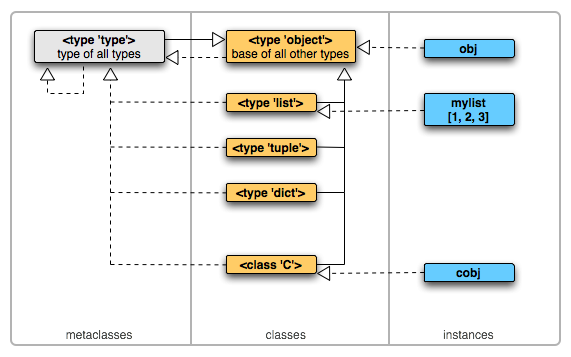
\includegraphics[height=4cm]{typesmap.png}
\end{minipage}




\subsubsection{Limitations of the reflective features}

\todo[inline]{TODO}



\newpage
\subsection{JavaScript}

\setjs
\subsubsection{Languages features for dealing with reflection and meta-programming}

Different informations about the type of an object \lstinline|custom| can be found in JavaScript :
\begin{itemize}
\item The primitive data type of an object can be found using the \lstinline|typeof| operator (e.g. \lstinline|typeof custom // "object"|)

\item To access the function that created the object, the \lstinline|custom.constructor| instruction can be used. (e.g. \lstinline|custom.constructor // function CustomObject()|)

\item The \lstinline|instanceof| operator allows to check if an object is an instance of a particular constructor (or has this constructor in its prototype chain). \\
		Example: \\
		\lstinline|custom instanceof CustomObject // true| \\
		\lstinline|custom instanceof Object // true|

		\smallskip
		N.B. objects created from primitive data type are considered as instances of \lstinline|Object| : \\
		\lstinline|new Boolean() instanceof Object; // true| \\
		\lstinline|new String() instanceof Object; // true| \\
		\lstinline|new Number() instanceof Object; // true| \\
\end{itemize}


\paragraph{Undefined object}{
In the case of an \lstinline|undefined| object, only the primitive data type can be retrieved (i.e. \lstinline|typeof undefined // "undefined"|), as the \lstinline|Undefined| constructor is not defined, and an \lstinline|undefined| object has no properties.
}


\paragraph{Object properties}{
It is possible to get the own properties of the object \lstinline|s| by calling \lstinline|Object.getOwnPropertyNames(s)|. \\
Example:
\begin{lstlisting}
function Song (artist, title) {
    this.title  = title;
    this.artist = artist;
    this.display = function() {
        return artist+" - "+title;
    }
}
var s = new Song("Mark Knopfler", "What It Is");
print(Object.getOwnPropertyNames(s));
// Array ["title", "artist", "display"]
\end{lstlisting}
}


There is no built-in feature to get the methods of an object (as of ECMAScript 5.1). But it can be achieved by the following function :
\begin{lstlisting}
var getMethodNames = function(obj) {
    var methods = [];
    for (var i in obj) {
        if (obj[i] instanceof Function) {
            methods.push(i);
        }
    }
    return methods;
}
getMethodNames(s); // Array ["display"]
\end{lstlisting}


There are two ways to get the prototype of an object :
\begin{lstlisting}
Object.getPrototypeOf(s); // standard way
s.__proto__;
\end{lstlisting}


The prototype properties of a constructor can be accessed this way :
\begin{lstlisting}
Song.prototype.genre = "rock";
Song.prototype; // Object { genre: "rock", constructor: Song() }
\end{lstlisting}

It can also be retrieved from an object :
\begin{lstlisting}
s.constructor.prototype; // Object { genre: "rock", constructor: Song() }
\end{lstlisting}

So now, the object s has a field \lstinline|genre| :
\begin{lstlisting}
s.genre; // "rock"
\end{lstlisting}

JavaScript proceeds method lookup in the following order :
\begin{enumerate}
\item in the object itself;
\item following the prototype chain.
\end{enumerate}


\bigskip
JavaScript allows to define object properties reflectively :
\begin{lstlisting}
Object.getOwnPropertyNames(s);
// Array ["title", "artist", "display"]
s.hasOwnProperty("album"); // false
s.album = "Sailing to Philadelphia";
Object.getOwnPropertyNames(s);
// Array ["title", "artist", "display", "album"]
s.hasOwnProperty("album"); // true
s.album; // "Sailing to Philadelphia"
\end{lstlisting}

It is also possible to set object properties :
\begin{lstlisting}
s.title = "Why Worry";
s.album = "Brother In Arms";
\end{lstlisting}


\medskip
\label{bind}
The \lstinline|bind| method creates a new function which, when called, has its \lstinline|this| keyword set to the provided value. \\
Example (taken from the MDN) : \\
\begin{lstlisting}
this.x = 9;
var module = {
	x: 81,
	getX: function() { return this.x; }
};

module.getX(); // 81

var getX = module.getX;
getX(); // 9, because in this case, "this" refers to the global object

// Create a new function with 'this' bound to module
var boundGetX = getX.bind(module);
boundGetX(); // 81
\end{lstlisting}

As in JavaScript the value of this is determined by how a function is called, the \lstinline|bind| method is useful to set the value of a function’s \lstinline|this|, regardless of how it is called.
It is particularly useful when making AJAX requests.


The ECMAScript 6 proposal brings the \lstinline|Proxy| object.
It allows to define custom behavior for fundamental operations (e.g. property lookup, assignment, enumeration, function invocation, etc).
But it is not yet implemented in web browsers as of this writing. \\
Example (taken from the MDN) : \\
\begin{lstlisting}
var handler = {
    // Return 37 if 'name' is not in target
    get: function(target, name){
        return name in target?
            target[name] :
            37;
    }
};

var p = new Proxy({}, handler); // new Proxy(target, handler)
p.a = 1;
p.b = undefined;

console.log(p.a, p.b); // 1, undefined
console.log('c' in p, p.c); // false, 37
\end{lstlisting}



\subsubsection{Kinds of reflection and meta-programming features}

JavaScript allows different kinds of reflection features :
\begin{itemize}
    \item Introspection : looking at the reified entities.
    \item Intercession : changing the program behaviour by manipulating the reified entities.
\end{itemize}

As JavaScript is an interpreted language, it proceeds runtime reflection.
That means that the system can be adapted at runtime, once it has been created and run.



\subsubsection{Meta-object protocol}

The primitive data types in JavaScript are of type object (i.e. \lstinline|Object|, \mbox{\lstinline|Boolean|,} \lstinline|String|, \lstinline|Number|, and \lstinline|Symbol|).
% these are *not* instances of Object !
Everything is object in JavaScript, even objects’ prototypes.
Note that Functions are also objects.

The prototype object that has been used to create the object can be referenced by using the \lstinline|__proto__| property.
In the figure, the \lstinline|__proto__| property is used to link prototypes and to provide inheritance.
% foo.__proto__ == Foo.prototype // true

The \lstinline|prototype| property corresponds to the object that was used to build the actual object.

\begin{figure}[h]
    \centering
    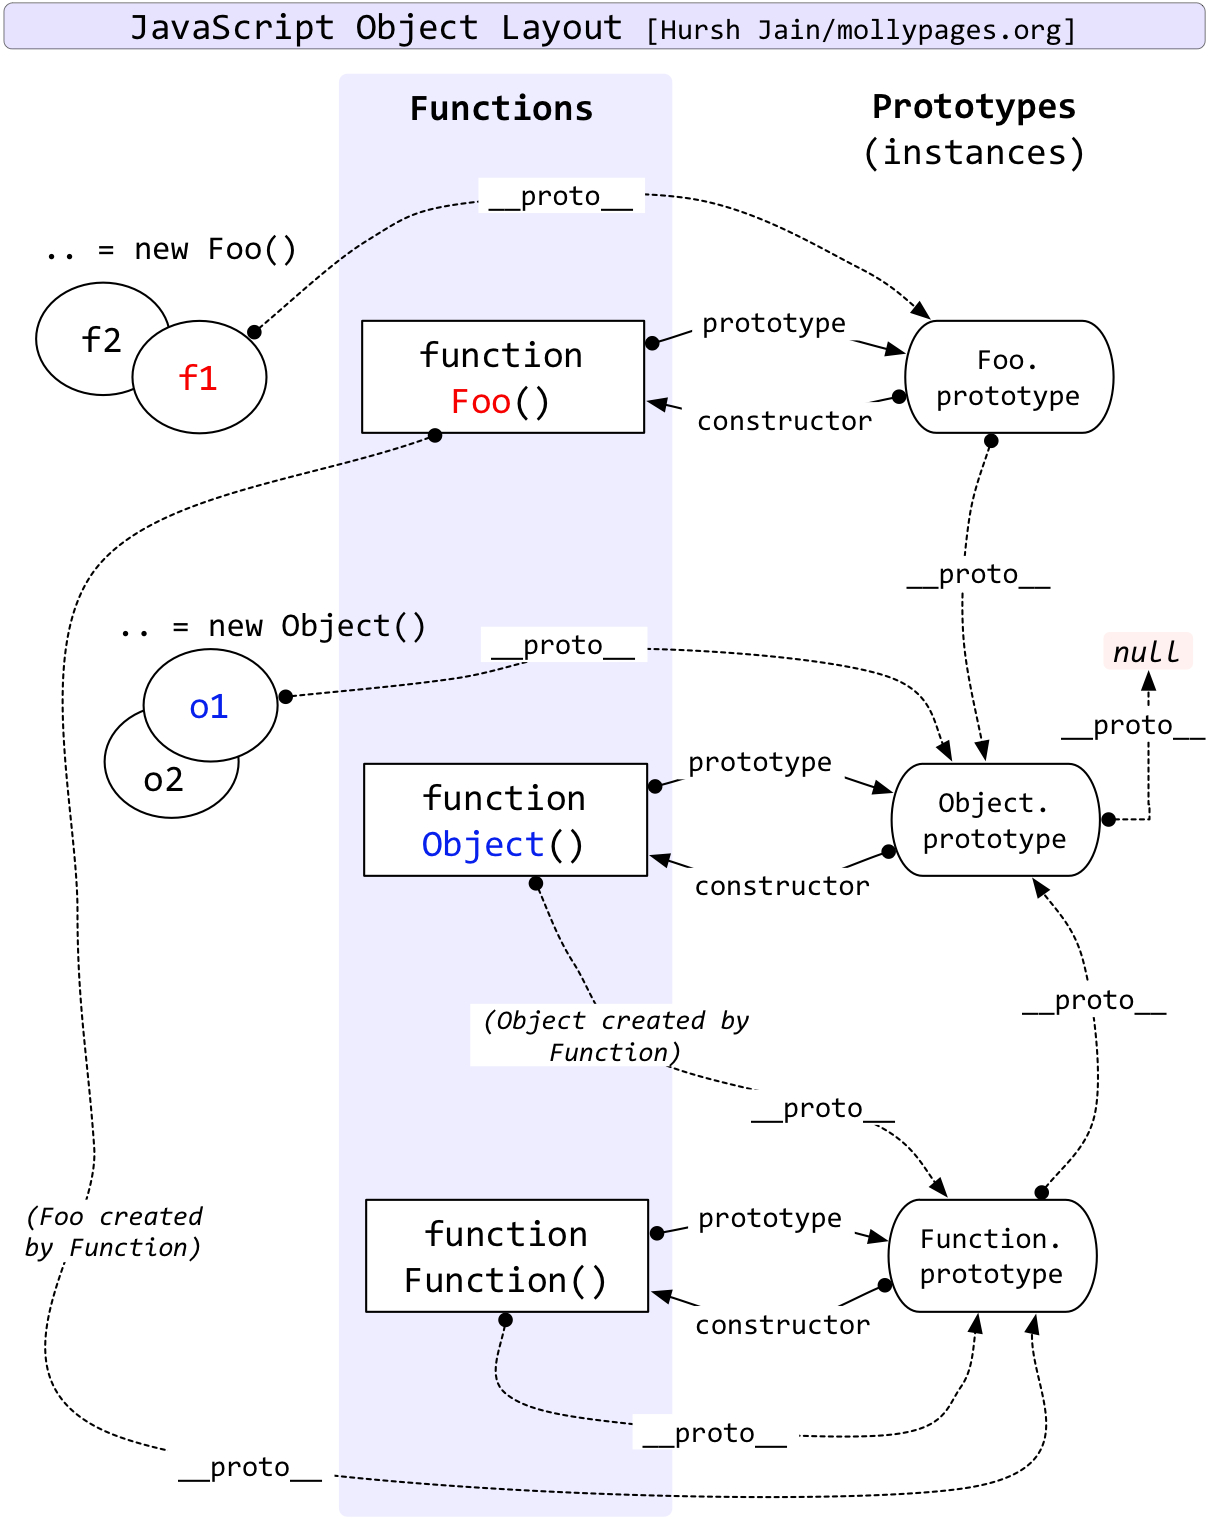
\includegraphics[width=0.5\textwidth]{jsobj_full.jpg}
\end{figure}

When the \lstinline|f1| object is created (with the \lstinline|new| keyword), its \textit{internal} \lstinline|__proto__| refers to the prototype of the \lstinline|Foo| function.
Therefore, \lstinline|Foo.prototype| \textit{inherits} from the prototype of \lstinline|Object|.
The \lstinline|__proto__| property can be used to provide \textit{inheritance} of properties.


\subsubsection{Limitations of the reflective features}

In JavaScript, object properties can be deleted, but not the objects themselves.
Contrarily to Ruby, there is no way to access instances of a constructor in JavaScript.




\newpage
\section{Comparing the languages}



\section{Conclusion}



\section{Bibliography}
\todo[inline]{Bibliography}


\end{document}
